\section{Passo 4 — Consolidar e ler o fluxo PRISMA}
\label{sec:passo4}

\subsection*{Objetivo}
Transformar documentos de bases diferentes em famílias comparáveis e medir quanto do volume inicial
era redundância.

\begin{figure}[H]
\centering
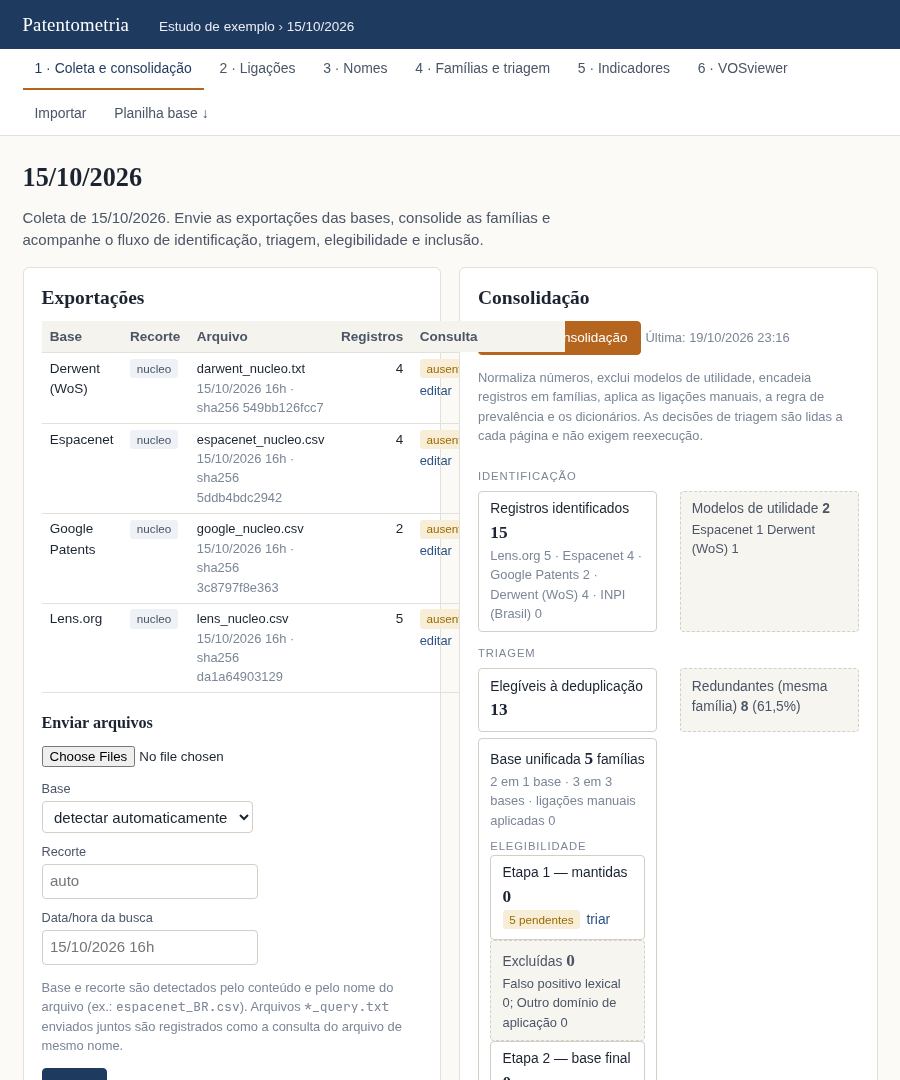
\includegraphics[width=0.8\linewidth]{img/04_rodada_topo.png}
\caption{Fluxo da rodada de demonstração: 15 documentos identificados, 2 modelos de utilidade
excluídos, 13 elegíveis e 5 famílias. O painel também mostra a distribuição por número de bases e o
que ainda está pendente na triagem.}
\label{fig:prisma}
\end{figure}

\subsection*{O que fazer}
\begin{enumerate}
\item Na rodada, clique em \textbf{Consolidar}.
\item Leia o fluxo de cima para baixo, conferindo cada subtotal.
\item Abra \textbf{Famílias} para ver o resultado da deduplicação.
\end{enumerate}

\subsection*{Como interpretar}
\begin{itemize}
\item \textbf{Identificados (15)}: documentos lidos, somando as quatro bases (5 + 4 + 2 + 4).
\item \textbf{Modelos de utilidade (2)}: documentos excluídos por tipo, antes da deduplicação.
\item \textbf{Elegíveis (13)}: identificados menos os excluídos por tipo.
\item \textbf{Redundantes (8, 61,5\%)}: documentos que representam invenções já contadas em outra
      família ou em outra base. É a medida do retrabalho que a deduplicação elimina.
\item \textbf{Base unificada (5)}: famílias efetivamente analisadas. O texto auxiliar mostra a
      distribuição: \num{3} famílias aparecem em três bases e \num{2} em apenas uma.
\item \textbf{Pendentes (5)}: famílias ainda sem decisão na etapa 1. Enquanto houver pendente, a
      base final não existe.
\end{itemize}

A distribuição por número de bases é um indicador de cobertura, não de qualidade: uma família
presente em três bases é mais robusta a erro de exportação; uma família exclusiva de uma base pode ser
uma lacuna das outras buscas. As exclusivas aparecem discriminadas por base --- na demonstração, uma
do Google e uma do Derwent.

\begin{nota}[Como citar o PRISMA]
Cite sempre o conjunto completo: ``15 documentos identificados, 2 excluídos por tipo, 13 elegíveis,
8 redundantes (61,5\%) e 5 famílias''. Dizer apenas ``5 famílias'' esconde o esforço de deduplicação e
impede a comparação com outras rodadas.
\end{nota}

\begin{alerta}[Erro comum]
Tratar ``famílias'' como ``patentes''. Uma família pode reunir pedido e concessão, em vários países;
contar documentos em vez de famílias infla qualquer série histórica.
\end{alerta}

\subsection*{Checkpoint}
\marcador\; Identificados $-$ modelos de utilidade $=$ elegíveis; elegíveis $-$ redundantes $=$ famílias;
e o número de pendentes da etapa 1 é igual ao número de famílias.
